\chapter{Testing and Evaluation}

\section{Testing}

Software testing is an investigation conducted to provide information about the quality of the product or service under test. Testing is executing a system in order to identify any gaps, errors, or missing requirements in contrary to the actual requirements. In my project I am using test-driven approach method, this helps eliminate parts of the code that will not work or fix them before adding them to system.

\subsection{Service testing}

As this project is Test Driven Development approach, all service unit testing has previously been done. These tests were done by building a small client application in Playground and web-server in Perfect which was developed and ran in Xcode. The API requests were tested afterwards using the Postman application, to run each API request and ensure the result is as expected. The tested included check the secret key and application key were authenticated, and if an incorrect key was used, then an error would be returned. Included bottom are some of the requests made along with the response in table \ref{tb:service-testing}.

\begin{table}[!h]
\centering
\caption{Service Testing}
\label{tb:service-testing}
\begin{tabular}{|c|c|c|l|l|}
\hline
\rowcolor{green!20}
\multicolumn{1}{|l|}{API Call}  & \multicolumn{1}{l|}{HTTP method} & \multicolumn{1}{l|}{Response}   & Body    & Result \\ \hline
\begin{tabular}[c]{@{}c@{}}http://perfectserver.site/api/\\ cc2b14fa-f59b-4e13-905a-3eebaf2ff659/\\ storage/RemoteConfig\end{tabular} & GET                                                      & Figure \ref{fig:api1}                                                                                                            &                                                                                                                                                     & PASS                           \\ \hline
\begin{tabular}[c]{@{}c@{}}http://perfectserver.site/\\ storage/TBAnalyitcs/\end{tabular}                                             & GET                                                      & \begin{tabular}[c]{@{}c@{}}\{,"result": "error"\\ ,"message": ""\}\end{tabular}                                             &                                                                                                                                                     & FAIL                           \\ \hline
\begin{tabular}[c]{@{}c@{}}http://perfectserver.site/api/\\ cc2b14fa-f59b-4e13-905a-3eebaf2ff659/\\ storage/Friends\end{tabular}      & GET                                                      & Figure \ref{fig:api2}                                                                                                            &                                                                                                                                                     & PASS                           \\ \hline
\begin{tabular}[c]{@{}c@{}}http://perfectserver.site/api/\\ cc2b14fa-f59b-4e13-905a-3eebaf2ff659/\\ storage/Friends\end{tabular}      & POST                                                     & \begin{tabular}[c]{@{}c@{}}\{,"result": "success",\\ "message":\\  "0e9635f6-b3fd-408d-\\ b4a2-458dab34c781"\}\end{tabular} & \begin{tabular}[c]{@{}l@{}}\{"dob": "12/12/2016",\\ "age": "44",\\ "name": "Jimmy"\\ ,"county": "Portsmouth"\\ ,"country": "England"\}\end{tabular} & \multicolumn{1}{c|}{PASS}      \\ \hline
\end{tabular}
\end{table}

\begin{figure}[!h]
    \caption{API Call 1}
    \centering
    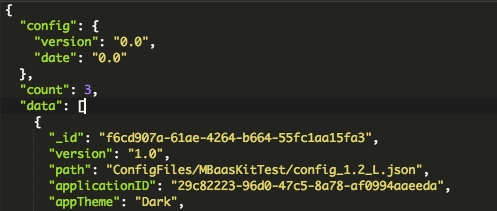
\includegraphics[width=100mm]{images/testing/api1}
    \label{fig:api1}
\end{figure} 

\begin{figure}[!h]
    \caption{API Call 2}
    \centering
    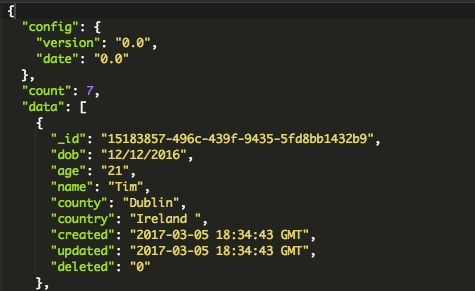
\includegraphics[width=100mm]{images/testing/api2}
    \label{fig:api2}
\end{figure} 

\newpage

\subsection{Integrated App Testing}

This part of testing involved developing a new mobile application with a simply user interface. The SDK developed was downloaded uses Cocoapods and installed in the testing app workspace. The application illustrated in the following figures \ref{fig:dark-theme} and \ref{fig:light-theme} , displays a table view where an array of "Friends" are displayed. The objective of created this test application is to demonstrate the remote configuration that allows the user to choose a new theme \ref{fig:app-themes-options} , and instantly see the difference.

The project aim from the beginning was to speed up development, testing and when the app is live. The figures \ref{fig:dark-theme} and \ref{fig:light-theme} illustrates how the app can be updated when the application is live quickly. The next three listings illustrate on what is required in the development stage to be able to update the UI objects when the app is published. 

In listing \ref{lst:test1} is UI objects include label and button, and these in one line can be initialised to start using the remote configuration feature.

\lstinputlisting[label={lst:test1},language=Swift, caption=Remote Config demo1]{testing_evaluation/code/test_project1.m}

In listing \ref{lst:test2} illustrates how the remote configuration file is being retrieved based on the theme chosen.

\lstinputlisting[label={lst:test2},language=Swift, caption=Remote Config demo2]{testing_evaluation/code/test_theme.m}

In listing \ref{lst:test2} the configuration file is being updated. This mean the old file is being deleted, and the new file updated to current main name and location. Next the navigation bar is being updated.

\lstinputlisting[label={lst:test3},language=Swift, caption=Remote Config demo3]{testing_evaluation/code/test_update.m}

\begin{figure}[!h]
    \caption{App Theme options}
    \centering
    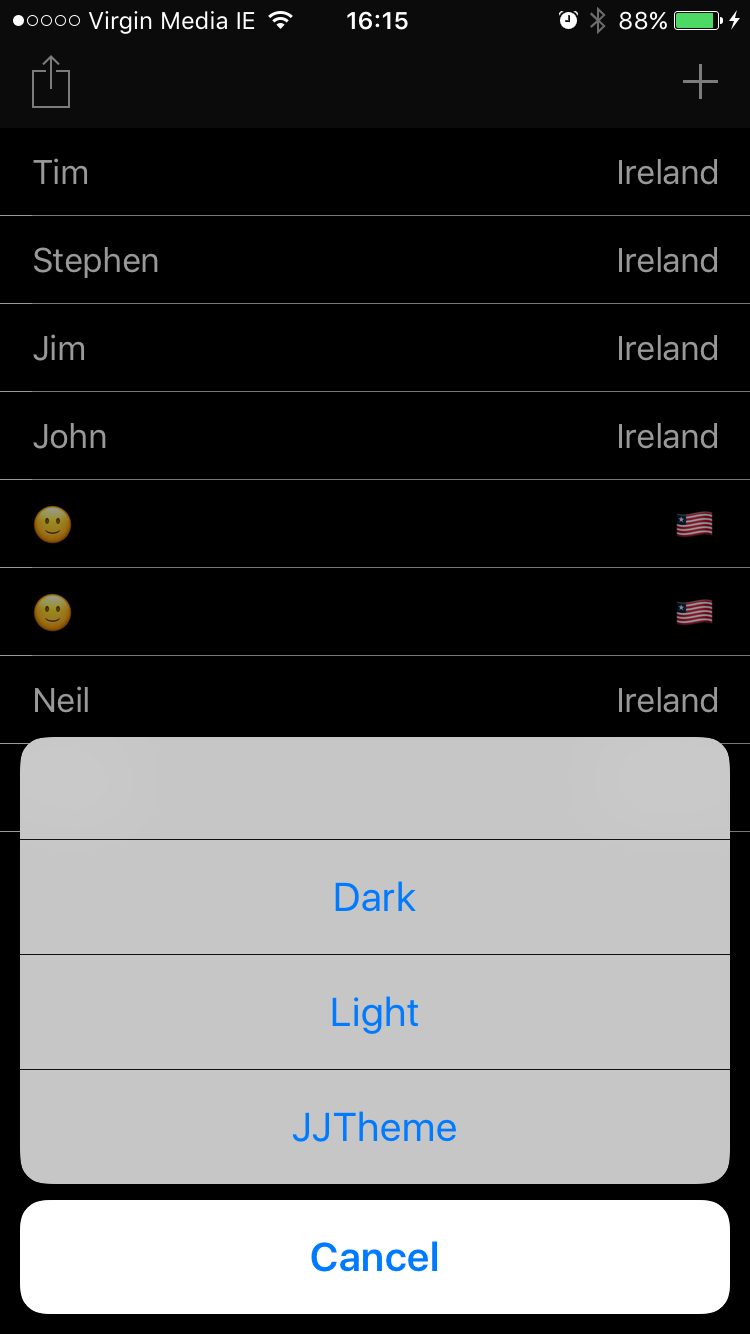
\includegraphics[width=60mm]{images/testing/themes}
    \label{fig:app-themes-options}
\end{figure} 

\begin{figure}[!h]
    \begin{subfigure}{0.5\textwidth}
        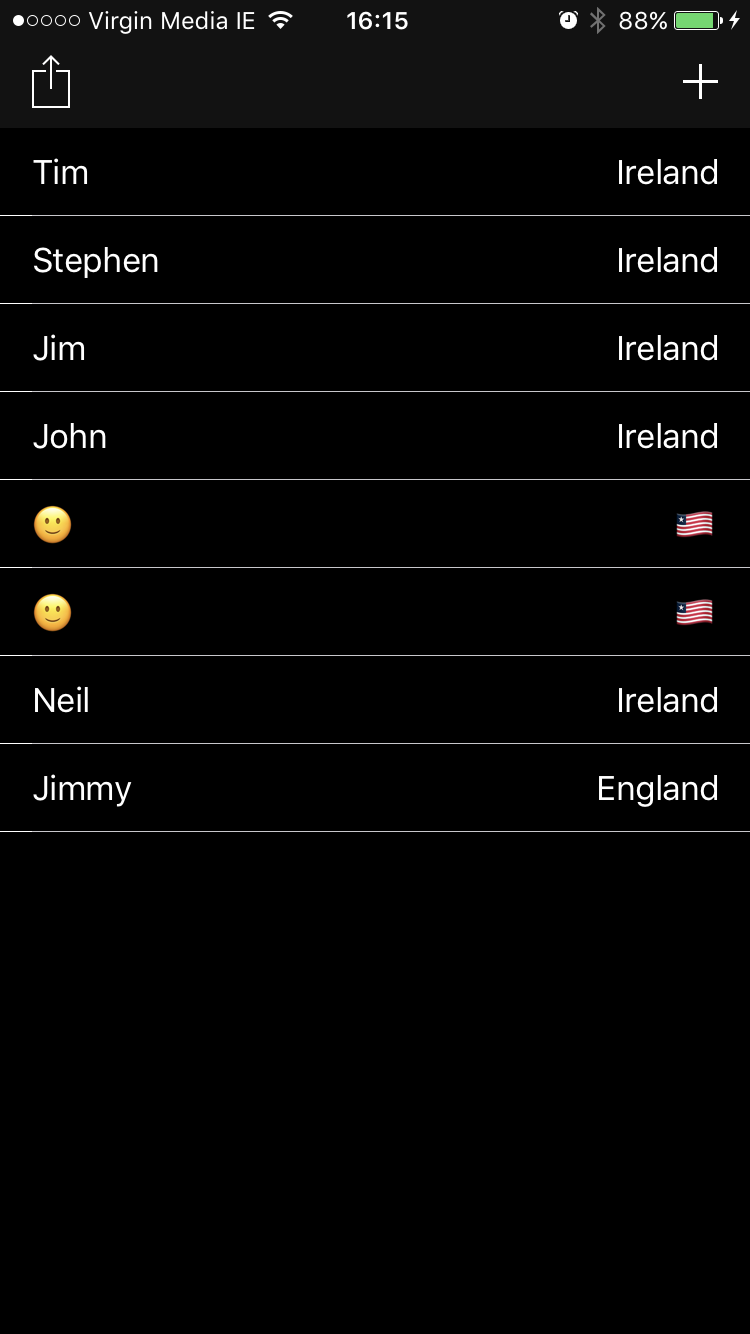
\includegraphics[width=0.8\linewidth, height=9cm]{images/testing/darkTheme}
        \caption{Dark Theme}
        \label{fig:dark-theme}
    \end{subfigure}
    \begin{subfigure}{0.5\textwidth}
        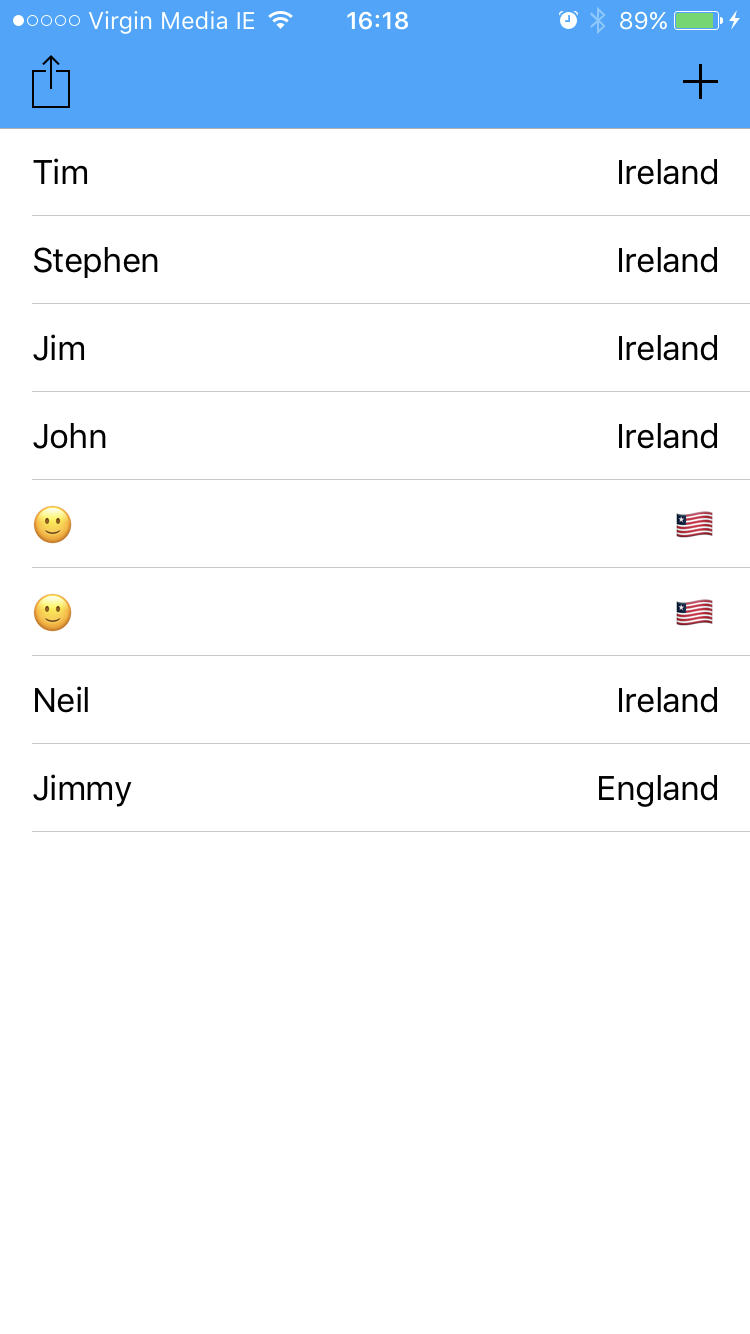
\includegraphics[width=0.8\linewidth, height=9cm]{images/testing/lightTheme}
        \caption{App Version}
        \label{fig:light-theme}
    \end{subfigure}
\caption{App Themes}
\label{fig:app-themes}
\end{figure}


\subsection{Sanity testing}

Sanity testing is kind of software testing which is performed once a build is completed with changes made. The goal is to run through the functionality in the application, and ensure they work as expected. Sanity testing is also carried out to check that the reported bugs fixed and new features does not break previously working functionality. The kind of testing is performed by testers which was done using college colleagues. A list of tests was given as seen in table \ref{tb:sanity} along with the average result found. The table \ref{tb:sanity} tests refers to the application stated above in integrated app testing section.

\begin{table}[!h]
\centering
\caption{Sanity testing 1}
\label{tb:sanity}
\begin{tabular}{|l|l|l|l|l|l|}
\hline
\rowcolor{green!20}
No & Description     & Initial state     & Steps                                                                                                   & Expected Result                                                                                                                 & Result \\ \hline
1  & Add new Friend  & App opened        & \begin{tabular}[c]{@{}l@{}}1. Selected add option\\ 2. Fill in details \\ 3. Press send\end{tabular}    & \begin{tabular}[c]{@{}l@{}}Friend has been added\\ and view returns to list of \\ friends view\end{tabular}                     & Pass   \\ \hline
2  & Update Friend   & Friends list view & \begin{tabular}[c]{@{}l@{}}1. Select friend to update\\ 2. Update values\\ 3. Press send\end{tabular}   & \begin{tabular}[c]{@{}l@{}}Friend is updated and view\\ returns to list of friends with\\ friend updated\end{tabular}           & Pass   \\ \hline
3  & Remove Friend   & Friends list view & \begin{tabular}[c]{@{}l@{}}1. Slide cell with friend\\ 2. Press delete\end{tabular}                     & \begin{tabular}[c]{@{}l@{}}Friend is deleted, and record\\ is gone\end{tabular}                                                 & Pass   \\ \hline
4  & Change Theme    & App opened        & \begin{tabular}[c]{@{}l@{}}1. Select icon at top left\\ 2. Choose theme ie. Dark\end{tabular}           & \begin{tabular}[c]{@{}l@{}}A pop up message stating \\ Dark Them downloaded, and \\ UI view is changed accordingly\end{tabular} & Pass   \\ \hline
5  & Change Language & App opened        & \begin{tabular}[c]{@{}l@{}}1. Select icon at top left\\ 2. Choose language\\   ie. English\end{tabular} & \begin{tabular}[c]{@{}l@{}}A pop up messaging stating\\ English downloaded, and title\\ bar caption is changed\end{tabular}     & Pass   \\ \hline
\end{tabular}
\end{table}

\section{Evaluation}

The evaluation was done by two outsourced developers from Trust5, by using the test example project. The evaluation feedback from both developers are included in the case chapter until section evaluation. The general feedback is good based the usability of the library, and how effortless using the library is. The developer also offered some constructive feedback where improvements can be made, such as expanding the documentation on the Github page, and possibly to make the library with Objective-C. 